\documentclass[11pt,a4paper]{article}

% ---------------------------------------------------------
% Packages
% ---------------------------------------------------------

\usepackage[utf8]{inputenc}
\usepackage[T1]{fontenc}
\usepackage[english]{babel}

\usepackage[
    a4paper,
    margin=2.5cm
]{geometry}

\usepackage{graphicx}
\usepackage{booktabs}
\usepackage{microtype}
\usepackage{amsmath}
\usepackage{url}
\usepackage[hidelinks]{hyperref}
\usepackage{caption}
\usepackage{tikz}

\usetikzlibrary{
    arrows.meta,
    positioning
}

\graphicspath{{figures/}}

\captionsetup{
    font=small,
    labelfont=bf
}

% Show only major sections in the table of contents.
% Subsections remain numbered in the document.
\setcounter{tocdepth}{1}

\hypersetup{
    pdftitle={
        Metadata-Aware Text-to-Spark-SQL
        for Cross-Source Data Lake Analytics
    },
    pdfauthor={Alessandro Schmitt}
}

% ---------------------------------------------------------
% Document
% ---------------------------------------------------------

\begin{document}

% ---------------------------------------------------------
% Title page
% ---------------------------------------------------------

\begin{titlepage}
\centering

\vspace*{1.2cm}

{\Large\textbf{Università degli Studi Roma Tre}\par}

\vspace{0.45cm}

{\large
Big Data --- Academic Year 2025/2026\par
}

\vspace{0.15cm}

{\large
Prof. Riccardo Torlone\par
}

\vfill

{\LARGE\bfseries
Metadata-Aware Text-to-Spark-SQL\\[0.2cm]
for Cross-Source Data Lake Analytics
\par}

\vspace{0.65cm}

{\Large First Project Report\par}

\vfill

\begin{tabular}{rl}
\textbf{Student:} & Alessandro Schmitt \\[0.15cm]
\textbf{Matricola:} & 577421
\end{tabular}

\vspace{1.2cm}

\end{titlepage}


% ---------------------------------------------------------
% Front matter
% ---------------------------------------------------------

\pagenumbering{roman}

\begin{abstract}

Natural-language analytics over heterogeneous data lakes requires a system to
identify not only the intended computation, but also the physical datasets,
columns, cross-source relationships, and semantic rules needed to express that
computation. This report presents a metadata-aware Text-to-Spark-SQL prototype
that combines a structured metadata catalog, semantic retrieval,
relation-aware expansion, SQL-safe context rendering, local language-model
generation, SQL validation, optional one-shot repair, and Apache Spark
execution.

The system is evaluated on a frozen 20-question held-out benchmark over NYC
taxi, geographic, and hourly weather data. Complete-catalog prompting achieves
70\% result accuracy, relation-aware retrieval improves accuracy to 80\%, and
validation with one-shot repair reaches 85\%. Relation-aware prompting also
reduces mean prompt size by 69.66\%, while controlled prompt-evaluation time
decreases by 70.29\% in the CPU-only experimental environment. Additional
experiments separate metadata scalability from physical data scalability:
catalog growth reveals a trade-off between bounded context size and retrieval
recall, while Spark workloads are evaluated from 100,000 to 2,963,713 curated
Yellow Taxi records.

\end{abstract}

\clearpage

\tableofcontents

\clearpage
\pagenumbering{arabic}


% ---------------------------------------------------------
% Main report
% ---------------------------------------------------------

\section{Introduction}
\label{sec:introduction}

\subsection{Motivation}

Modern data analytics increasingly relies on data lakes that integrate
multiple heterogeneous sources rather than on a single, centrally designed
relational database. Although this architecture simplifies the storage and
integration of large and diverse datasets, it also makes analytical access
more complex. A user who wants to formulate a cross-source query must know
which datasets are relevant, understand their schemas and semantics, identify
the relationships between them, and finally express the analysis using the
query language supported by the processing engine.

Large language models (LLMs) provide a promising interface for reducing this
complexity by translating natural-language analytical requests into SQL.
However, applying Text-to-SQL techniques directly to a heterogeneous data lake
introduces an additional problem: the model needs sufficient metadata to
identify the correct physical datasets, columns, relationships, and semantic
rules. Providing the complete metadata catalog for every query is simple, but
it can introduce large amounts of irrelevant information and causes the prompt
to grow as the catalog grows. Moreover, a metadata catalog may contain
semantic concepts, aliases, relationship identifiers, and descriptive rules
that are useful for retrieval but are not valid physical SQL identifiers.

This project investigates an alternative approach in which the metadata
provided to the LLM is selected dynamically for each user question. The goal
is to preserve the information required for correct query generation while
avoiding the cost and ambiguity of exposing the complete catalog.


\subsection{Problem Statement}

The project considers a heterogeneous data lake containing New York City
urban-mobility and weather data. The core sources are NYC TLC Yellow Taxi trip
records, NYC TLC Green Taxi trip records, NYC Taxi Zones, and hourly weather
observations. These datasets differ in schema, granularity, semantics, and
analytical role, while meaningful user requests may require relationships
across multiple sources.

For example, a request concerning the borough with the largest number of taxi
pickups during rainy hours requires more than simply identifying columns whose
names are similar to words in the question. The system must identify the taxi
trip dataset, the pickup-location relationship with the Taxi Zones dataset,
the temporal relationship with hourly weather observations, and the semantic
condition used to represent a rainy hour. The generated query must then use
the corresponding physical Spark SQL tables and columns rather than internal
metadata identifiers.

The central challenge is therefore to determine how much metadata should be
provided to the language model and how that metadata should be represented.
Too little information may cause the model to omit a required dataset,
relationship, or semantic rule. Too much information increases prompt size and
may expose irrelevant or misleading metadata.


\subsection{Proposed Approach}

The implemented system follows a metadata-aware Text-to-Spark-SQL pipeline.
A structured metadata catalog describes datasets, physical columns, semantic
concepts, aliases, cross-source relationships, and reusable semantic rules.
Metadata documents are indexed using vector embeddings so that candidate
metadata can be retrieved from a natural-language question.

The initial semantic retrieval is then expanded using explicit relationships
stored in the catalog. This relation-aware expansion makes it possible to add
the physical endpoints required for joins even when they are not directly
retrieved by semantic similarity. The selected metadata is subsequently
rendered into a SQL-safe context that exposes only executable physical table
and column names, join conditions, and SQL expressions to the language model.

A local LLM generates Spark SQL from this restricted context. The resulting
query is parsed and validated before execution. If validation fails, the
system can perform a single repair attempt using the validation error together
with the same retrieved metadata context. Valid queries are finally executed
using Apache Spark SQL over the curated data lake.


\subsection{Research Question}

The main research question investigated in this work is:

\begin{quote}
\emph{To what extent can dynamic, relation-aware metadata retrieval improve
the correctness and efficiency of Text-to-Spark-SQL generation over a
heterogeneous data lake compared with providing the complete metadata catalog
to the language model?}
\end{quote}

The evaluation considers both correctness and efficiency. Correctness is
measured at the metadata-retrieval and query-result levels, while efficiency is
evaluated through prompt size, controlled inference latency, catalog growth,
and Spark execution under increasing data volume.


\subsection{Contributions}

The main contributions of the project are the following:

\begin{itemize}

    \item A reproducible metadata-aware Text-to-Spark-SQL prototype for
    cross-source analytics over a heterogeneous Spark-based data lake.

    \item A structured metadata catalog containing physical schemas, semantic
    concepts, aliases, cross-source relationships, and SQL-oriented semantic
    rules.

    \item A relation-aware retrieval strategy that combines semantic retrieval
    with deterministic metadata expansion and produces a restricted,
    SQL-safe context for the language model.

    \item A validation and one-shot repair stage that prevents invalid SQL
    from being executed directly and attempts to recover from generation
    errors without changing the retrieved metadata.

    \item A frozen held-out evaluation comparing three configurations:
    complete-catalog prompting, relation-aware metadata retrieval, and
    relation-aware retrieval with validation and repair.

    \item Separate scalability experiments for metadata-catalog growth and
    physical data volume, allowing catalog scalability and Spark execution
    scalability to be analysed independently.

\end{itemize}


\subsection{Summary of Results}

On the frozen held-out benchmark, the complete-catalog baseline achieved
70\% result accuracy. Relation-aware metadata retrieval increased result
accuracy to 80\%, while the addition of validation and one-shot repair reached
85\%. At the same time, relation-aware prompting reduced the mean prompt size
from 2558.45 to 776.35 tokens, corresponding to a 69.66\% reduction.

A separate controlled latency experiment showed that the smaller
relation-aware prompt reduced mean prompt-evaluation time from 182.58 seconds
to 54.24 seconds in the evaluated CPU-only local environment, a reduction of
70.29\%.

The catalog-scaling experiment showed that the full metadata context increased
from 9,498 characters with four sources to 16,651 characters with sixteen
sources, whereas the mean retrieved context remained close to 2,100
characters. This increased compression was accompanied by a measurable
retrieval trade-off: macro recall decreased from 0.925 to 0.825 after
semantically related hard-negative sources were introduced and then remained
stable when the catalog was further expanded.

Finally, Spark data-volume experiments evaluated the same workloads from
100,000 rows up to the full Yellow Taxi dataset of 2,963,713 curated records.
These experiments complement the catalog-scale evaluation by measuring the
system along the physical data-volume dimension rather than the metadata
dimension.

The remainder of this report describes the data sources, metadata model,
system architecture, implementation, experimental methodology, results, and
limitations in detail.

\section{Background and Project Requirements}

\section{Data Lake and Datasets}
\label{sec:data-lake}

\subsection{Data-Lake Scope}

The experimental data lake was constructed around New York City
urban-mobility analytics for January 2024. The core catalog contains four
physical datasets: Yellow Taxi trip records, Green Taxi trip records, Taxi
Zones, and hourly weather observations.

The choice deliberately combines datasets with different analytical roles.
Yellow and Green Taxi contain high-volume transactional trip records, Taxi
Zones provides geographic reference data, and the weather source provides a
temporal environmental dimension. As a consequence, answering cross-source
questions requires the system to reconcile different schemas and
granularities rather than querying a single homogeneous table.

All datasets used by Spark were curated into Parquet before the
Text-to-Spark-SQL experiments. The metadata layer therefore describes a
stable curated representation rather than exposing the language model
directly to raw source files.


\subsection{Yellow Taxi Trip Records}

The Yellow Taxi dataset is the largest source in the project and represents
the main data-volume component of the experimental setting. The January 2024
raw input contained 2,964,624 records. After curation, 2,963,713 records were
retained with 19 physical columns.

The dataset includes pickup and drop-off timestamps, pickup and drop-off
location identifiers, trip distance, fare-related attributes, and other
operational fields. In the metadata catalog, the physical Spark table is
registered as \texttt{yellow\_taxi}.

The pickup timestamp,
\texttt{tpep\_pickup\_datetime}, is particularly important for cross-source
analytics because it provides the temporal reference used to associate a
trip with the corresponding hourly weather observation. Similarly,
\texttt{PULocationID} and \texttt{DOLocationID} provide the physical keys
used to connect taxi trips with geographic information from the Taxi Zones
dataset.


\subsection{Green Taxi Trip Records}

The Green Taxi dataset provides a second trip-record source with a similar
analytical domain but a different physical schema. The January 2024 raw input
contained 56,551 records, of which 56,429 remained after curation. The
curated representation contains 20 physical columns and is registered in
Spark as \texttt{green\_taxi}.

Although Yellow and Green Taxi describe related events, they cannot be
treated as a single identical schema. In particular, their pickup and
drop-off timestamp columns use different physical names. Green Taxi uses
\texttt{lpep\_pickup\_datetime} for the pickup timestamp, whereas Yellow
Taxi uses \texttt{tpep\_pickup\_datetime}. This difference illustrates the
role of semantic metadata: both fields represent the same general concept
of a pickup time while remaining distinct physical SQL columns.

As for Yellow Taxi, Green Taxi location identifiers can be related to Taxi
Zones, while the pickup timestamp can be converted to an hourly bucket and
related to the weather source.


\subsection{Taxi Zones}

Taxi Zones is a compact geographic reference dataset containing 265 rows and
4 physical columns. It maps a numeric \texttt{LocationID} to descriptive
geographic attributes including zone and borough information.

Despite its small physical size, Taxi Zones is essential for many analytical
questions. Taxi-trip records store location identifiers rather than
human-readable geographic names. Therefore, a question such as ``Which
borough received the largest number of Green Taxi drop-offs?'' requires a
join between the transactional trip source and the zone reference source.

The project explicitly models four taxi-to-zone relationships: Yellow pickup,
Yellow drop-off, Green pickup, and Green drop-off. Distinguishing pickup from
drop-off relationships is necessary because both are represented by location
identifiers but correspond to different analytical meanings.


\subsection{Hourly Weather}

The weather source provides the temporal environmental dimension used for
questions involving rain, temperature, and hourly conditions. The curated
January 2024 dataset contains 744 hourly buckets and 23 columns.

Of the 744 expected hourly positions for the month, 743 contain an observed
weather record. One hourly bucket is explicitly represented as missing rather
than silently removed. The curated data contains 167 rainy hours and 576 dry
hours, with one hour whose precipitation status remains unknown because of
the missing observation.

Weather observations are registered in Spark as
\texttt{weather\_hourly}. The physical \texttt{weather\_hour} column is the
temporal key used for joins. Taxi pickup timestamps are converted to hourly
granularity using \texttt{date\_trunc('hour', ...)} before being compared
with this field.

Precipitation semantics are normalized during curation. Positive
precipitation values are treated as rainy conditions. Trace precipitation is
also considered precipitation even though no positive numeric amount can be
assigned to it. A zero precipitation amount represents a dry observation,
while missing precipitation information is kept distinct from both rainy and
dry conditions.


\subsection{Data Curation}

Curation was performed before metadata indexing and query generation so that
all downstream experiments operate over stable physical datasets.

For the taxi sources, records were restricted to pickups occurring in January
2024. Rows with missing pickup or drop-off timestamps were removed, and a
drop-off was required to occur after its corresponding pickup. Pickup and
drop-off location identifiers were required to correspond to valid taxi-zone
identifiers. Trip distance was constrained to non-negative values not
exceeding 1,000 miles.

The curation procedure intentionally avoids applying overly aggressive domain
assumptions. Zero-distance trips are preserved, as are negative monetary
values and zero passenger counts when they are present in the source data.
These values can represent unusual but potentially meaningful operational
records and were therefore not removed merely because they appear
counter-intuitive.

For weather data, raw observations were normalized to one record per clock
hour. When multiple observations were available within the same hourly
bucket, the preferred observation type was selected when available, with a
deterministic fallback to the latest suitable observation. The resulting
representation provides a stable hourly temporal key for cross-source joins.


\subsection{Cross-Source Relationships}

The metadata catalog explicitly represents six relationships required by the
core data lake.

Four relationships connect taxi locations to Taxi Zones:

\begin{itemize}

    \item \texttt{yellow\_taxi.PULocationID} to
    \texttt{taxi\_zones.LocationID};

    \item \texttt{yellow\_taxi.DOLocationID} to
    \texttt{taxi\_zones.LocationID};

    \item \texttt{green\_taxi.PULocationID} to
    \texttt{taxi\_zones.LocationID};

    \item \texttt{green\_taxi.DOLocationID} to
    \texttt{taxi\_zones.LocationID}.

\end{itemize}

Two additional relationships connect taxi pickup times with hourly weather:

\begin{itemize}

    \item
    \texttt{date\_trunc('hour',
    yellow\_taxi.tpep\_pickup\_datetime)}
    to \texttt{weather\_hourly.weather\_hour};

    \item
    \texttt{date\_trunc('hour',
    green\_taxi.lpep\_pickup\_datetime)}
    to \texttt{weather\_hourly.weather\_hour}.

\end{itemize}

These relationships are stored as metadata rather than being inferred by the
language model for every request. This allows relation-aware retrieval to
expand an initially selected dataset or column into the physical join
endpoints required for execution.


\subsection{Volume and Variety in the Experimental Data}

The data lake represents the two Big Data dimensions selected for this
project.

\emph{Volume} is primarily provided by the taxi-trip datasets and is evaluated
experimentally using progressively larger subsets of Yellow Taxi data, from
100,000 records to the complete curated set of 2,963,713 records.

\emph{Variety} arises from the combination of transactional mobility data,
geographic reference data, and hourly weather observations. The sources have
different schemas, column naming conventions, row granularities, and
relationships. This heterogeneity motivates the metadata-aware architecture:
a natural-language request can refer to one conceptual analytical task while
its execution requires physical fields distributed across multiple datasets.

\section{Metadata-Aware Architecture}
\label{sec:architecture}

\subsection{Architecture Overview}

The proposed system transforms a natural-language analytical request into an
executable Spark SQL query through a sequence of metadata-aware stages. The
architecture separates metadata selection, language-model generation,
validation, and physical query execution.

The complete processing flow is:

\begin{enumerate}

    \item receive a natural-language analytical question;

    \item retrieve metadata that is semantically relevant to the question;

    \item expand the initial metadata selection using semantic concepts,
    aliases, dataset evidence, and explicit cross-source relationships;

    \item render the selected metadata into a restricted SQL-safe context;

    \item ask a local language model to generate one Spark SQL query;

    \item parse and validate the generated SQL against the registered Spark
    schema and the expected output structure;

    \item if validation fails, optionally perform one repair attempt using the
    validation feedback and the same metadata context;

    \item execute the valid query using Spark SQL and return the computed
    result.

\end{enumerate}

The architecture is deliberately not implemented as a multi-agent system.
Deterministic Python orchestration is used for metadata processing,
validation, repair control, and Spark execution. The LLM is used only where
natural-language interpretation and SQL generation are required.



Figure~\ref{fig:system-architecture} summarizes the complete processing
pipeline and the separation between metadata grounding, generation,
validation, and execution.

\begin{figure}[htbp]
\centering

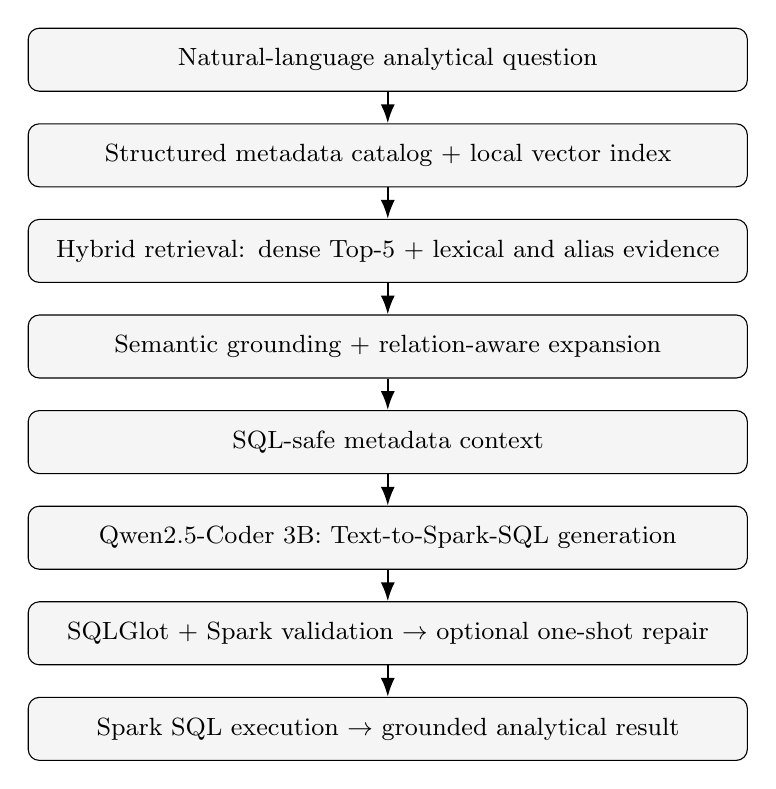
\begin{tikzpicture}[
    node distance=4mm,
    stage/.style={
        draw,
        rounded corners,
        align=center,
        text width=0.73\textwidth,
        minimum height=8mm,
        inner sep=4pt,
        font=\small,
        fill=gray!8
    },
    flow/.style={
        -{Latex[length=2.4mm]},
        thick
    }
]

\node[stage] (question)
    {Natural-language analytical question};

\node[stage, below=of question] (catalog)
    {Structured metadata catalog + local vector index};

\node[stage, below=of catalog] (retrieval)
    {Hybrid retrieval:
    dense Top-5 + lexical and alias evidence};

\node[stage, below=of retrieval] (expansion)
    {Semantic grounding + relation-aware expansion};

\node[stage, below=of expansion] (renderer)
    {SQL-safe metadata context};

\node[stage, below=of renderer] (llm)
    {Qwen2.5-Coder 3B:
    Text-to-Spark-SQL generation};

\node[stage, below=of llm] (validation)
    {SQLGlot + Spark validation
    $\rightarrow$ optional one-shot repair};

\node[stage, below=of validation] (spark)
    {Spark SQL execution
    $\rightarrow$ grounded analytical result};

\draw[flow] (question) -- (catalog);
\draw[flow] (catalog) -- (retrieval);
\draw[flow] (retrieval) -- (expansion);
\draw[flow] (expansion) -- (renderer);
\draw[flow] (renderer) -- (llm);
\draw[flow] (llm) -- (validation);
\draw[flow] (validation) -- (spark);

\end{tikzpicture}

\caption{
End-to-end metadata-aware Text-to-Spark-SQL architecture.
}
\label{fig:system-architecture}
\end{figure}

\subsection{Structured Metadata Catalog}

The metadata catalog is the central source of structural and semantic
knowledge used by the system. It is implemented as a relational SQLite
catalog and describes the curated Spark datasets rather than the original raw
files.

The core catalog contains four datasets and 66 physical columns. In addition
to the physical schema, it stores 21 semantic concepts, 29 column-to-concept
associations, 6 explicit relationships, 27 aliases, and 6 reusable semantic
rules.

The catalog separates several kinds of information:

\begin{itemize}

    \item \textbf{datasets}, including descriptions, physical paths,
    granularity, temporal information, and row counts;

    \item \textbf{columns}, representing the physical fields that can appear
    in executable Spark SQL;

    \item \textbf{semantic concepts}, providing a common vocabulary across
    heterogeneous physical schemas;

    \item \textbf{aliases}, connecting natural-language variants to datasets,
    concepts, and schema elements;

    \item \textbf{relationships}, describing executable join conditions
    between datasets;

    \item \textbf{semantic rules}, representing reusable SQL predicates or
    expressions associated with analytical concepts.

\end{itemize}

This separation allows semantic knowledge to be used during retrieval without
assuming that every metadata identifier is also a valid SQL identifier.


\subsection{Metadata Vector Index}

To support semantic retrieval, metadata entities are transformed into textual
documents and embedded using the local \texttt{embeddinggemma} model.

The base catalog produces 103 indexed metadata documents:

\begin{itemize}

    \item 66 column documents;
    \item 21 semantic-concept documents;
    \item 4 dataset documents;
    \item 6 relationship documents;
    \item 6 semantic-rule documents.

\end{itemize}

The resulting 768-dimensional embeddings are stored in a local Qdrant vector
index using cosine similarity.

The vector index is not used as an independent knowledge base. Its purpose is
to identify semantically promising metadata entities from the natural-language
question. Structural completeness is handled by the subsequent deterministic
expansion stage.


\subsection{Hybrid Metadata Retrieval}

The retrieval procedure combines dense semantic retrieval with deterministic
lexical and metadata-based evidence.

For each question, the system first retrieves the top five dense metadata
candidates from the vector index. Dense retrieval is complemented by lexical
matching against physical names and aliases. Explicit dataset mentions in the
question are treated as strong evidence and can override unrelated dataset
candidates returned only by embedding similarity.

Semantic concepts can also be expanded to their associated physical columns.
For example, a general concept such as pickup time can correspond to
\texttt{yellow\_taxi.tpep\_pickup\_datetime} or
\texttt{green\_taxi.lpep\_pickup\_datetime}, depending on the dataset
identified by the question.

The retrieval stage therefore does not simply select the five nearest vector
documents. Dense similarity is used as one signal inside a broader
metadata-grounding procedure.


\subsection{Relation-Aware Expansion}

Cross-source analytical queries often require metadata that is not directly
similar to the wording of the user question. A join key such as
\texttt{LocationID}, for example, may be essential for execution even if the
question mentions only a borough name.

To address this issue, the system performs deterministic relationship
expansion after the initial metadata retrieval. When selected datasets imply a
known catalog relationship, the relationship and its physical endpoint
columns can be added to the metadata selection.

Relationship selection also considers the query wording. This is necessary
when multiple relationships connect the same pair of datasets. Taxi records,
for example, can be related to Taxi Zones through either pickup or drop-off
location identifiers. Evidence in the question is therefore used to
distinguish pickup-oriented and drop-off-oriented relationships.

A similar mechanism is used for temporal relations between taxi pickups and
hourly weather observations. The catalog stores the executable relationship
between the hourly bucket derived from the taxi pickup timestamp and
\texttt{weather\_hourly.weather\_hour}.

This stage is one of the main differences between ordinary semantic retrieval
and the proposed relation-aware approach.


\subsection{Semantic Rules}

Some analytical concepts cannot be represented by selecting a physical column
alone. The catalog therefore contains semantic rules that associate common
analytical meanings with executable Spark SQL expressions or predicates.

For example, a rainy hour is represented by the physical predicate

\begin{verbatim}
weather_hourly.has_precipitation = TRUE
\end{verbatim}

while the taxi pickup hour is represented using an hourly transformation of
the corresponding pickup timestamp.

Rules are included in the retrieved context only when the selected metadata
and question provide evidence that they are relevant. This prevents the model
from receiving every semantic rule in the catalog for every request.


\subsection{SQL-Safe Context Rendering}

The metadata selected by retrieval cannot be passed directly to the language
model because the internal catalog contains identifiers that are meaningful
for metadata management but are not executable SQL.

The SQL-safe renderer therefore transforms the selected metadata into a
restricted prompt context. It exposes:

\begin{itemize}

    \item physical Spark table names;

    \item fully qualified physical column names;

    \item natural-language descriptions of their meaning;

    \item executable physical join conditions;

    \item executable SQL expressions and predicates.

\end{itemize}

Internal semantic-concept identifiers, relationship names, rule identifiers,
and aliases are not exposed as if they were physical SQL objects.

This distinction is important because the complete-catalog baseline contains
both physical and semantic metadata. Without SQL-safe rendering, an LLM can
incorrectly use an internal semantic identifier as a table or column name.

The renderer also provides dataset-level temporal information. Since the
registered taxi and weather datasets already contain only January 2024 data,
the context explicitly informs the model that an additional January predicate
is unnecessary unless the user requests a narrower date range.


\subsection{Text-to-Spark-SQL Generation}

The SQL generation component uses the local
\texttt{qwen2.5-coder:3b} model through Ollama \cite{hui2024qwen25coder}. Generation is deterministic,
with temperature set to zero and a context window of 4096 tokens.

The model receives the natural-language question together with either the full
catalog context or the relation-aware SQL-safe context, depending on the
experimental configuration.

Its task is restricted to generating a Spark SQL query. The model does not
directly compute the analytical answer. This ensures that final numerical
results are obtained from the physical datasets through Spark rather than from
the parametric knowledge of the language model.


\subsection{SQL Validation}

Generated SQL is validated before execution using a dedicated validation
stage.

The validator performs three main checks:

\begin{enumerate}

    \item parse the query using SQLGlot with the Spark SQL dialect;

    \item ensure that the generated statement is a single read-only query and
    that it references only allowed physical tables;

    \item ask Spark to analyse the query against the registered physical
    schemas and verify the expected output columns.

\end{enumerate}

This design catches syntactic errors, unknown tables, unknown physical
columns, and several forms of invalid schema grounding before actual query
execution.

Validation does not prove semantic correctness. A syntactically valid query
can still express the wrong analytical intention, which is why final
evaluation is based on query results rather than validation success alone.


\subsection{One-Shot SQL Repair}

When validation fails, the third system configuration allows one repair
attempt.

The repair model receives the invalid SQL, the validation feedback, the
original question, and the same retrieved metadata context used during the
initial generation. No gold SQL or expected answer is provided to the repair
stage.

Restricting repair to a single attempt keeps the experimental configuration
simple and prevents an uncontrolled iterative agent loop. If the repaired
query still fails validation, the system reports the failure instead of
continuing indefinitely.

The repair mechanism is intended to correct generation errors when the
required metadata is already available. It cannot recover information that
was omitted by the retrieval stage. This distinction becomes important in the
held-out error analysis.


\subsection{Spark SQL Execution and Grounded Results}

After successful validation, the query is executed using Apache Spark SQL over
the curated Parquet datasets.

Spark is therefore the authoritative computational layer of the system.
Aggregations, filters, joins, grouping operations, and result values are all
computed from the stored data.

The final architecture separates responsibilities clearly:

\begin{itemize}

    \item the metadata catalog represents structural and semantic knowledge;

    \item the retrieval layer selects the context required for a question;

    \item the LLM translates the grounded request into Spark SQL;

    \item validation checks whether the generated query is executable;

    \item optional repair handles a limited class of generation errors;

    \item Spark computes the final analytical result.

\end{itemize}

This separation also enables the experimental evaluation to analyse retrieval
quality, SQL correctness, LLM efficiency, catalog scalability, and Spark
data-volume scalability as distinct components of the overall system.

\section{Implementation}
\label{sec:implementation}

\subsection{Technology Stack}

The prototype is implemented primarily in Python and uses Apache Spark as the
structured data-processing engine.

The main technologies are:

\begin{itemize}

    \item \textbf{Python 3.12} for orchestration, catalog management,
    retrieval, validation, experimental evaluation, and reporting;

    \item \textbf{PySpark 3.5.8} and \textbf{Java 17} for Spark SQL execution
    over the curated Parquet data lake;

    \item \textbf{SQLite} for the persistent structured metadata catalog;

    \item \textbf{Qdrant} in local embedded mode for vector-based metadata
    retrieval;

    \item \textbf{Ollama} for running both the embedding model and the local
    Text-to-SQL language model;

    \item \texttt{embeddinggemma} for metadata embeddings;

    \item \texttt{qwen2.5-coder:3b} for Spark SQL generation and optional
    one-shot repair;

    \item \textbf{SQLGlot} for SQL parsing and dialect-aware validation;

    \item \textbf{Matplotlib} for generation of reproducible report figures.

\end{itemize}

All language-model inference is executed locally. No paid external model API
is required by the final prototype.


\subsection{Execution Environment}

The implementation and experiments were executed in a GitHub Codespaces
environment based on Ubuntu Linux.

Spark runs locally using two worker threads. The principal experimental
configuration uses:

\begin{verbatim}
--master local[2]
--driver-memory 1g
\end{verbatim}

Spark SQL uses four shuffle partitions in the controlled data-volume
benchmark, while adaptive query execution is enabled.

The local execution environment is intentionally modest. It contains two CPU
cores and no dedicated GPU. This constraint is relevant when interpreting
language-model latency results: the measured inference times describe the
CPU-only experimental environment and are not intended as general performance
claims for the underlying model.


\subsection{Repository Organization}

The implementation is organized into separate directories for configuration,
source code, scripts, datasets, and experimental artifacts.

The principal structure is:

\begin{verbatim}
config/
data/
  raw/
  curated/
  catalog/
artifacts/
  benchmarks/
  report/
scripts/
  catalog/
  data/
  experiments/
  reporting/
  retrieval/
src/
  metadata_agent/
report/
\end{verbatim}

The \texttt{src/metadata\_agent} package contains reusable application
components such as the catalog access layer, metadata document construction,
embedding support, relation-aware retrieval, SQL validation, and repair
logic.

The \texttt{scripts/} hierarchy contains reproducible entry points for data
preparation, metadata indexing, validation, experimental evaluation, and
final report artifact generation.

Configuration files are stored separately under \texttt{config/}. This keeps
experimental inputs, such as benchmark questions and synthetic catalog-scale
distractors, outside the implementation code.


\subsection{Curated Data Storage}

Raw source data and curated analytical datasets are stored separately.

The curated Spark datasets are written in Parquet format. This choice provides
a columnar representation directly supported by Spark SQL and avoids requiring
a separate database server for physical query execution.

The main curated paths correspond to January 2024 Yellow Taxi, Green Taxi,
Taxi Zones, and hourly weather data. These physical paths are recorded in the
metadata catalog together with schema, row-count, temporal, and semantic
information.

Generated raw and curated datasets are excluded from Git version control
because they are reproducible and potentially large. Experimental benchmark
summaries and final report artifacts, in contrast, are committed to the
repository.


\subsection{Metadata Catalog Implementation}

The metadata catalog is materialized as a SQLite database. Its content is
constructed from a versioned configuration file and the actual curated Spark
schemas.

The core tables include:

\begin{itemize}

    \item \texttt{datasets};
    \item \texttt{columns};
    \item \texttt{semantic\_concepts};
    \item \texttt{column\_semantics};
    \item \texttt{relationships};
    \item \texttt{aliases};
    \item \texttt{semantic\_rules};
    \item \texttt{catalog\_meta}.

\end{itemize}

Physical column definitions are checked against the curated Parquet schemas
during catalog construction. This reduces the risk of maintaining metadata
that refers to schema elements that do not exist in the execution layer.

The generated SQLite file is treated as a reproducible artifact rather than a
source file and is therefore excluded from Git.


\subsection{Metadata Document Construction and Embedding}

The vector index does not embed the complete catalog as a single document.
Instead, individual metadata entities are converted into separate textual
documents.

One document is generated for each physical column, semantic concept, dataset,
relationship, and semantic rule. The base configuration therefore produces
103 independently retrievable documents.

Each document includes enough natural-language description to support
semantic matching while its payload preserves the corresponding metadata
entity type and key.

Embeddings are produced locally using \texttt{embeddinggemma}. The resulting
768-dimensional vectors are inserted into a Qdrant collection using cosine
distance.

The index can be rebuilt deterministically from the metadata catalog and is
therefore not committed as a binary repository artifact.


\subsection{Relation-Aware Retrieval Implementation}

The relation-aware retriever is implemented as a deterministic Python
component.

For each question it combines:

\begin{enumerate}

    \item dense Top-\(k\) retrieval from Qdrant, with \(k=5\);

    \item lexical matching against metadata names and aliases;

    \item semantic-concept expansion toward physical columns;

    \item dataset selection using explicit and inferred evidence;

    \item relationship selection and endpoint expansion;

    \item semantic-rule expansion when supported by the selected metadata.

\end{enumerate}

Explicit dataset mentions receive stronger priority than unrelated dense
retrieval candidates. This prevents a semantically similar but physically
different dataset from replacing a dataset named directly by the user.

Relationship selection also uses query evidence to distinguish alternatives.
For example, pickup-oriented and drop-off-oriented relationships connect the
same taxi source with the same Taxi Zones source but require different
physical columns.

The retrieval implementation returns both a structured metadata selection and
a rendered SQL-safe context. This makes it possible to evaluate retrieval
quality independently from downstream LLM generation.


\subsection{SQL-Safe Context Rendering}

The renderer converts the internal metadata selection into the text included
in the LLM prompt.

The implementation explicitly distinguishes between metadata identifiers and
physical Spark SQL identifiers. Internal concept names, alias names,
relationship identifiers, and rule identifiers are not presented as if they
were executable columns or tables.

Physical schema objects are rendered using fully qualified names whenever
appropriate. Join metadata is rendered as executable physical conditions, and
semantic rules are rendered as executable predicates or expressions.

The renderer also adds constraints explaining that the registered January
2024 tables are already temporally restricted. This avoids encouraging the
model to invent an unnecessary year or month column when no narrower date
filter is requested.


\subsection{Local LLM Configuration}

Text-to-Spark-SQL generation is performed through Ollama using
\texttt{qwen2.5-coder:3b}.

The generation parameters are fixed to:

\begin{itemize}

    \item temperature \(=0\);
    \item context size \(=4096\) tokens.

\end{itemize}

The deterministic temperature setting reduces sampling variability between
benchmark runs.

The same model is used for the complete-catalog baseline and for the
relation-aware configurations. As a result, the main A/B comparison changes
the metadata context rather than the language model.

The repair configuration also uses the same local model, but its prompt
contains the failed SQL and validator feedback in addition to the original
question and retrieved context.


\subsection{SQL Validation Implementation}

Validation is implemented using both SQLGlot and Spark.

SQLGlot first parses the generated query using the Spark dialect. The
validator then checks that the request contains a single read-only query and
that referenced tables belong to the allowed physical dataset set.

Spark analysis provides the second validation layer. Because Spark resolves
the query against the registered schemas, it can identify physical problems
such as unknown columns, unknown relations, incompatible expressions, and
other analysis errors.

The benchmark also associates each question with an expected output schema.
This allows the validator to detect cases in which the generated query returns
the wrong result structure even if its SQL is otherwise executable.


\subsection{One-Shot Repair Implementation}

Repair is implemented as a separate component rather than as an unrestricted
conversation loop.

A repair is attempted only after validation failure. The repair prompt
contains:

\begin{itemize}

    \item the original natural-language question;

    \item the metadata context used for the original generation;

    \item the invalid SQL query;

    \item the validation error returned by the validator.

\end{itemize}

Only one repaired SQL candidate is generated. The candidate is passed through
the same validation stage before any execution is attempted.

This implementation deliberately prevents repair from using the gold query or
gold result. It therefore tests whether validator feedback and already
available metadata are sufficient to recover from a generation error.


\subsection{Benchmark Configuration}

Benchmark questions and gold specifications are stored as versioned JSON
configuration files.

Each benchmark item can include:

\begin{itemize}

    \item the natural-language question;

    \item required datasets;

    \item required physical columns;

    \item required relationships;

    \item required semantic rules;

    \item expected output columns;

    \item gold Spark SQL;

    \item gold result information.

\end{itemize}

This representation supports evaluation at multiple levels. Metadata
retrieval can be compared with the required metadata set, while generated SQL
can be validated and ultimately compared by result rather than only by exact
query text.


\subsection{Experimental Artifact Management}

Experimental outputs are written under \texttt{artifacts/benchmarks} as JSON
or text files. These files contain the final numerical results used by the
report.

Temporary execution logs and rebuildable indexes are stored separately and
excluded from version control.

The final reporting pipeline reads only the frozen benchmark JSON files. It
generates six figures in both PDF and PNG format and four summary tables in
both LaTeX and CSV format. It does not rerun Spark, Ollama, retrieval, or any
experimental benchmark.

This separation ensures that report generation cannot modify the underlying
experimental measurements.


\subsection{Reproducibility Strategy}

Reproducibility is supported at three levels.

First, the environment and Python dependencies are explicitly versioned,
including PySpark, SQLGlot, Qdrant client libraries, and Matplotlib.

Second, benchmark configurations, experiment scripts, and generated summary
results are committed to Git.

Third, the project uses Git tags to separate experimental protocol freezes
from observed results. Important evaluation stages were therefore committed
and tagged before the corresponding benchmark was executed.

This strategy is discussed in more detail in
Appendix~\ref{sec:reproducibility}.

\section{Experimental Methodology}
\label{sec:methodology}

\subsection{Evaluation Goals}

The experimental evaluation was designed to answer four related questions.

First, the study evaluates whether relation-aware metadata retrieval improves
Text-to-Spark-SQL correctness compared with providing the complete metadata
catalog to the language model.

Second, it measures whether metadata selection reduces the amount of prompt
context and the corresponding model-evaluation cost.

Third, it studies the behaviour of the retrieval layer when the metadata
catalog grows and contains semantically related distractor sources.

Fourth, it evaluates the Spark execution layer under increasing physical data
volume.

These goals deliberately separate two different notions of scalability:
\emph{catalog scale}, which concerns the number of metadata sources available
to the retrieval system, and \emph{data scale}, which concerns the number of
physical records processed by Spark.


\subsection{Development Benchmark}

An initial benchmark of ten analytical intents was used during development.
The questions cover single-source aggregation, filtering, geographic joins,
cross-taxi comparisons, temporal joins with weather data, and multi-source
queries involving both geographic and weather information.

Each benchmark item contains a gold specification including the metadata
required to answer the question. Depending on the analytical intent, this can
include required datasets, physical columns, relationships, and semantic
rules. The benchmark also contains a gold Spark SQL query and the expected
result.

The initial benchmark was used while implementing and correcting the
retrieval logic. Consequently, after this tuning activity it was explicitly
treated as a \emph{development set} and was not used as the main evidence for
generalisation performance.

This distinction is important because retrieval behaviour had already been
observed on these questions while the architecture was still being modified.


\subsection{Architecture Freeze}

Before the final held-out evaluation, the metadata-aware architecture was
frozen.

The frozen implementation includes:

\begin{itemize}

    \item metadata catalog access;
    \item metadata document construction;
    \item local embedding support;
    \item dense and lexical retrieval;
    \item semantic-concept expansion;
    \item dataset grounding;
    \item relation-aware expansion;
    \item semantic-rule expansion;
    \item SQL-safe context rendering;
    \item SQL validation;
    \item one-shot repair.

\end{itemize}

After this freeze, the retrieval architecture was not tuned using the final
held-out results. Git tags were used to preserve the exact implementation
state associated with each evaluation phase.


\subsection{Frozen Held-Out Benchmark}

A separate held-out benchmark was constructed after the development
architecture had been frozen.

The held-out benchmark contains 20 natural-language questions, with two new
paraphrases for each of the ten analytical intents represented in the
development set. The wording of these questions was not used to tune the
retriever before the benchmark was frozen.

The underlying gold analytical specification for each intent remains fixed:
the expected datasets, columns, relationships, semantic rules, output schema,
gold SQL, and gold result correspond to the same intended computation.
However, the natural-language formulation is new.

The held-out benchmark itself was committed and tagged before the first final
A/B/C system evaluation. This provides a clear separation between benchmark
definition and result observation.


\subsection{Experimental Configurations}

The main Text-to-Spark-SQL experiment compares three configurations.

\paragraph{Configuration A: Full Catalog.}

Configuration A is the baseline. The language model receives the complete
rendered metadata catalog for every question. No metadata retrieval is used to
restrict the catalog before generation.

This baseline represents the straightforward strategy of exposing all
available metadata to the model. It also preserves internal semantic catalog
information that is useful for describing the data but is not necessarily a
physical SQL identifier.

The generated SQL is validated before execution, but no repair attempt is
performed.

\paragraph{Configuration B: Relation-Aware Retrieval.}

Configuration B uses the proposed metadata retrieval architecture. Dense and
lexical evidence identify candidate metadata, after which semantic and
relationship expansion add structurally required entities.

Only the selected metadata is rendered into the SQL-safe context. The same
language model and generation parameters used by Configuration A are then used
to generate Spark SQL.

The generated SQL is validated before execution, but no repair attempt is
performed.

\paragraph{Configuration C: Retrieval with Validation and Repair.}

Configuration C uses the same relation-aware retrieval and SQL-safe context as
Configuration B.

The difference is that, when the initially generated SQL fails validation, the
system can perform one repair attempt using the validator feedback. If the
query is already valid, no repair is triggered.

This design isolates the incremental contribution of one-shot repair from the
contribution of metadata retrieval.


\subsection{Controlled Generation Configuration}

All A/B/C Text-to-Spark-SQL experiments use the same local
\texttt{qwen2.5-coder:3b} model through Ollama.

The principal generation parameters are fixed to:

\begin{itemize}

    \item temperature \(=0\);
    \item context size \(=4096\) tokens.

\end{itemize}

Using the same model and deterministic temperature across configurations
reduces the number of variables changed by the A/B comparison. The primary
difference between A and B is therefore the metadata context supplied to the
model.


\subsection{Metadata Retrieval Metrics}

Metadata retrieval is evaluated independently from SQL generation.

For each held-out query, the selected metadata entities are compared with the
gold required-metadata set.

The evaluation uses:

\begin{itemize}

    \item \textbf{recall}, measuring the fraction of required metadata entities
    successfully retrieved;

    \item \textbf{precision}, measuring the fraction of retrieved metadata
    entities that belong to the gold required set;

    \item \textbf{F1}, combining precision and recall;

    \item \textbf{perfect-recall queries}, counting questions for which all
    required metadata entities are present;

    \item \textbf{context size}, measured in characters;

    \item \textbf{context reduction}, measured relative to the complete
    catalog context;

    \item \textbf{retrieval latency}.

\end{itemize}

Gold metadata can contain physical datasets, columns, relationships, and
semantic rules. As a consequence, retrieval evaluation measures structural
completeness rather than only nearest-neighbour relevance.


\subsection{Text-to-Spark-SQL Metrics}

Generated SQL is evaluated at multiple levels.

\textbf{Validation rate} measures how often the generated query passes the
parser, read-only constraints, physical schema analysis, and expected-output
checks.

\textbf{Execution rate} measures how often a generated query can be executed
successfully using Spark.

The principal correctness metric is \textbf{result accuracy}. A generated
query is considered correct when its executed result matches the expected
gold result under the benchmark comparison procedure.

Result accuracy is preferred over exact SQL-string matching because different
SQL formulations can express the same computation. Conversely, a query can be
syntactically valid and executable while still returning the wrong analytical
result. Validation success is therefore not treated as a substitute for
semantic correctness.


\subsection{Prompt-Efficiency Metrics}

Prompt efficiency is evaluated by measuring the metadata-dependent input
provided to the local model.

The held-out A/B experiment records mean prompt-token count for both the
complete-catalog baseline and the relation-aware configuration.

The relative token reduction is calculated as:

\[
R_{\mathrm{tokens}}
=
1 -
\frac{T_B}{T_A},
\]

where \(T_A\) is the mean prompt-token count for the full-catalog baseline and
\(T_B\) is the mean count for relation-aware prompting.

Retrieval latency is measured separately so that the cost of metadata
selection is not hidden inside the LLM timing.


\subsection{Controlled Latency Protocol}

The original held-out execution revealed that model prompt-evaluation timing
can be strongly influenced by runtime cache effects. In particular, repeated
full-catalog prompts share a large common prefix, which can make later
requests appear artificially inexpensive.

For this reason, intrinsic A/B prompt cost is evaluated using a separate
controlled latency benchmark rather than relying only on the sequential
held-out timings.

Three representative held-out questions with perfect metadata recall were
selected:

\begin{itemize}

    \item one simple single-source analytical request;

    \item one taxi--weather temporal query;

    \item one three-source query involving taxi, geography, and weather.

\end{itemize}

Each A/B condition is executed twice in the controlled phase. A unique
prefix-isolation header is inserted before the otherwise frozen prompt
structure so that reuse of an identical long prefix is reduced.

The benchmark records prompt-token count, prompt-evaluation time, generation
time, API duration, and wall-clock time.

A separate natural-cache phase executes the exact prompts without the
isolation header. These measurements are retained to illustrate the practical
effect of prefix reuse, but the prefix-isolated measurements are used as the
primary latency comparison.

Model cold-load time is measured separately and is not mixed with the
warm-model prompt-evaluation comparison.


\subsection{Repair Evaluation}

Repair is evaluated only when Configuration C encounters an initially invalid
query.

The benchmark records:

\begin{itemize}

    \item the number of repair attempts;

    \item the number of repaired queries that pass validation;

    \item whether a repaired query improves final result accuracy.

\end{itemize}

A repair is not attempted for a query that is already valid. Consequently,
the repair mechanism cannot correct a semantically incorrect query that passes
validation.

Likewise, repair cannot reliably recover from missing metadata if the
retrieval stage failed to supply the physical schema or relationship required
for the intended computation.


\subsection{Catalog-Scale Experiment}

A separate experiment evaluates metadata retrieval as the catalog grows.

Three catalog sizes are considered:

\begin{itemize}

    \item 4 sources: the original physical data lake;

    \item 8 sources: the original catalog plus 4 metadata-only hard-negative
    sources;

    \item 16 sources: the original catalog plus 12 metadata-only
    hard-negative sources.

\end{itemize}

The additional sources are deliberately semantically related to the original
urban-mobility, geographic, and weather domain. They include concepts such as
alternative trip data, borough information, daily weather, transportation,
traffic, and environmental observations.

These sources are metadata-only distractors: no additional physical Spark data
is executed in this experiment. The purpose is to increase catalog ambiguity
while keeping the analytical gold answers unchanged.

The distractor specification and the evaluation harness were frozen before
the first catalog-scale run. No retrieval tuning was performed after observing
the 4/8/16-source results.

For each scale, a new metadata index is built and the same 20 frozen held-out
questions are evaluated with the same dense Top-\(5\) retrieval setting.

The experiment records:

\begin{itemize}

    \item number of datasets, columns, and metadata documents;

    \item complete-catalog context size;

    \item mean retrieved-context size;

    \item perfect-recall query count;

    \item macro precision, recall, and F1;

    \item mean context reduction;

    \item retrieval latency;

    \item metadata-index construction cost.

\end{itemize}


\subsection{Catalog-Scale Error Analysis}

After the catalog-scale results had been frozen, failures were analysed by
comparing the missing and extra metadata entities at 4, 8, and 16 sources.

This analysis is descriptive rather than corrective. The retrieval logic was
not modified in response to the observed failures.

The purpose of this analysis is to identify whether a loss of recall is caused
by general catalog growth or by competition from particular semantically
similar hard-negative metadata.


\subsection{Data-Volume Scaling Experiment}

Catalog growth and physical data growth are evaluated separately.

The data-volume benchmark uses the curated Yellow Taxi dataset and four row
counts:

\begin{itemize}

    \item 100,000 rows;
    \item 500,000 rows;
    \item 1,000,000 rows;
    \item the complete 2,963,713-row curated Yellow Taxi dataset.

\end{itemize}

Each scale is materialized outside the timed query execution as a two-file
Parquet dataset. The number of partitions is therefore held constant across
the measured scales.

Three Spark SQL workloads are evaluated:

\begin{enumerate}

    \item a scan with aggregate statistics;

    \item grouping by pickup zone;

    \item a temporal join between Yellow Taxi pickups and hourly weather.

\end{enumerate}

Each workload is executed three times for every scale. Scale order is
alternated between repetitions to reduce systematic ordering effects, and no
DataFrame is intentionally cached by the benchmark.

The principal reported timing is the median of the three repetitions. Median
runtime is used because short local Spark workloads are sensitive to
one-time JVM, filesystem, and execution warm-up effects.

The benchmark also records physical Parquet size and runtime relative to the
100,000-row baseline.


\subsection{Interpretation Constraints}

The experiments are intended to evaluate the implemented prototype, not to
establish universal performance claims for Spark, Qwen, Qdrant, or the
underlying embedding model.

In particular, language-model latency is specific to the CPU-only Codespaces
environment, and the Spark data-volume experiment is limited to approximately
three million Yellow Taxi records on two local worker threads.

Similarly, the catalog-scale distractors are a controlled set of
domain-related hard negatives rather than a complete simulation of an
enterprise metadata catalog.

The results are therefore interpreted as evidence about the behaviour and
trade-offs of the proposed architecture under the defined experimental
conditions.

\section{Experimental Results}
\label{sec:results}

\subsection{Held-Out Text-to-Spark-SQL Performance}

The main held-out evaluation compares the three configurations defined in
Section~\ref{sec:methodology} over 20 frozen natural-language questions.

Table~\ref{tab:heldout-abc} reports validation rate, execution rate, result
accuracy, and the absolute number of correct queries.

\begin{table}[htbp]
\centering
\caption{Held-out Text-to-Spark-SQL evaluation.}
\label{tab:heldout-abc}
\begin{tabular}{lrrr}
\toprule
Metric & A Full & B Retrieval & C Repair \\
\midrule
Validation rate & 75\% & 85\% & 90\% \\
Execution rate & 75\% & 85\% & 90\% \\
Result accuracy & 70\% & 80\% & 85\% \\
Correct queries & 14/20 & 16/20 & 17/20 \\
\bottomrule
\end{tabular}
\end{table}


Figure~\ref{fig:heldout-abc} presents the same comparison graphically.

\begin{figure}[htbp]
    \centering
    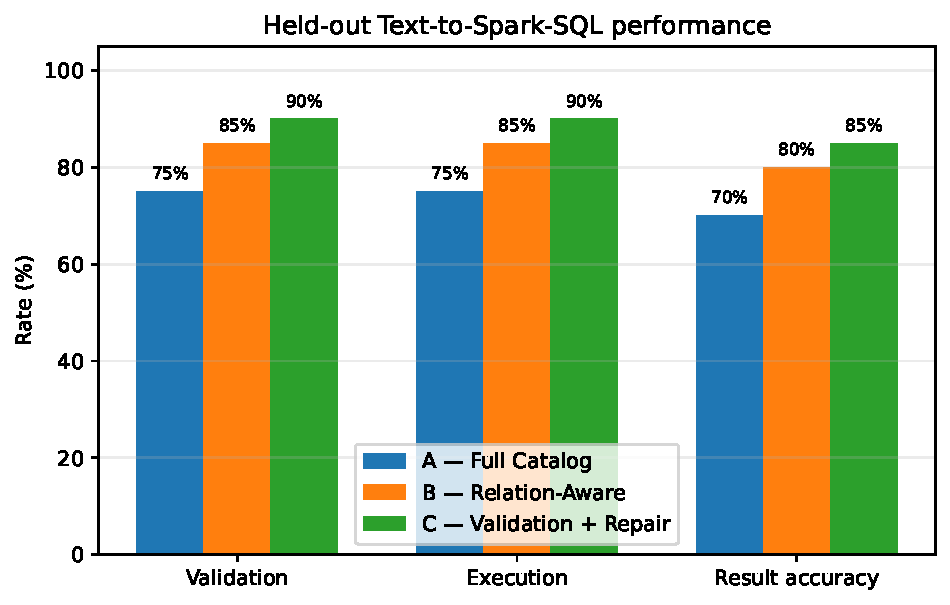
\includegraphics[
        width=0.82\textwidth
    ]{heldout_abc_rates.pdf}
    \caption{
        Held-out Text-to-Spark-SQL performance for configurations A, B, and C.
    }
    \label{fig:heldout-abc}
\end{figure}

The complete-catalog baseline, Configuration A, achieves a validation rate of
75\%, an execution rate of 75\%, and a final result accuracy of 70\%. This
corresponds to 14 correct results out of 20 held-out questions.

Replacing the complete metadata catalog with relation-aware SQL-safe metadata
retrieval improves all three metrics. Configuration B reaches 85\% validation,
85\% execution, and 80\% result accuracy, corresponding to 16 correct results
out of 20.

Configuration C adds validation-driven one-shot repair and obtains the highest
final performance: 90\% validation, 90\% execution, and 85\% result accuracy,
or 17 correct results out of 20.

The improvement from A to B is particularly important because both
configurations use the same language model and deterministic generation
parameters. The main experimental difference is therefore the metadata context
supplied before SQL generation.

The results indicate that reducing the catalog to a relation-aware SQL-safe
subset does not merely reduce prompt size. Under the held-out benchmark, it
also improves final query correctness.


\subsection{Prompt Efficiency}

The metadata-retrieval configuration substantially reduces the amount of
context supplied to the language model.

Table~\ref{tab:efficiency-latency} summarizes prompt-size and controlled
latency measurements.

\begin{table}[htbp]
\centering
\caption{Prompt-size and controlled-latency comparison.}
\label{tab:efficiency-latency}
\begin{tabular}{lrrr}
\toprule
Metric & A Full & B Retrieval & Reduction \\
\midrule
Mean prompt tokens & 2558.45 & 776.35 & 69.66\% \\
Prompt evaluation (s) & 182.58 & 54.24 & 70.29\% \\
Wall-clock time (s) & 202.31 & 69.29 & 65.75\% \\
\bottomrule
\end{tabular}
\end{table}


On the 20 held-out questions, Configuration A uses an average of 2558.45 prompt
tokens, while Configuration B uses 776.35 tokens. The relation-aware approach
therefore reduces mean prompt size by 69.66\%.

Figure~\ref{fig:prompt-tokens} highlights this reduction.

\begin{figure}[htbp]
    \centering
    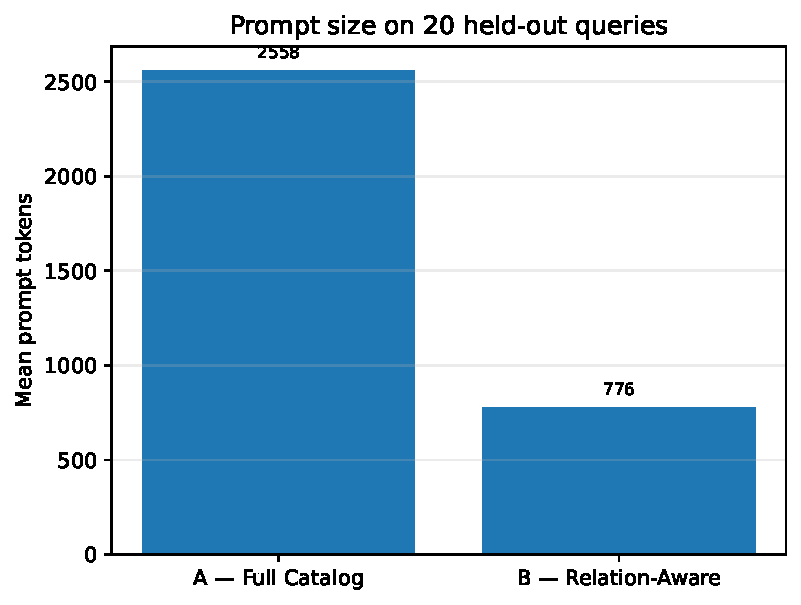
\includegraphics[
        width=0.68\textwidth
    ]{prompt_token_efficiency.pdf}
    \caption{
        Mean prompt-token count for complete-catalog and relation-aware
        prompting on the held-out benchmark.
    }
    \label{fig:prompt-tokens}
\end{figure}

The reduction is achieved without changing the underlying LLM. It results from
selecting only metadata considered relevant to the current analytical request
and rendering that metadata using physical SQL-safe identifiers.

This result supports one of the main motivations of the project: as metadata
catalogs grow, sending the complete catalog for every natural-language request
is not necessary for the evaluated workload.


\subsection{Controlled Inference Latency}

The sequential held-out execution exhibited strong cache effects, especially
for the complete-catalog prompts that repeatedly share a large common prefix.
For this reason, the primary latency comparison uses the controlled
prefix-isolated benchmark described in Section~\ref{sec:methodology}.

The controlled experiment reports a mean prompt-evaluation time of
182.58 seconds for Configuration A and 54.24 seconds for Configuration B.
This corresponds to a 70.29\% reduction in prompt-evaluation time.

Mean wall-clock time decreases from 202.31 seconds to 69.29 seconds, a
65.75\% reduction.

Figure~\ref{fig:controlled-latency} shows the controlled prompt-evaluation
comparison.

\begin{figure}[htbp]
    \centering
    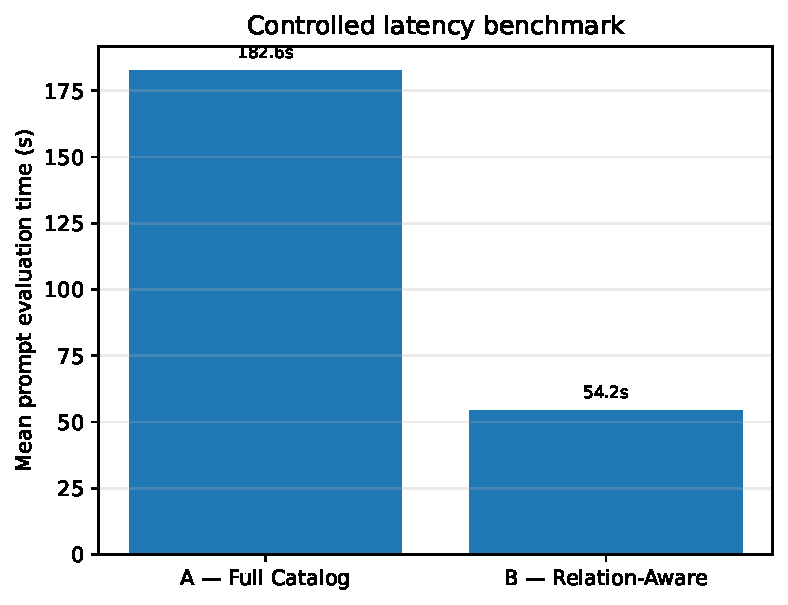
\includegraphics[
        width=0.68\textwidth
    ]{controlled_latency_prompt_eval.pdf}
    \caption{
        Mean controlled prompt-evaluation latency for complete-catalog and
        relation-aware prompting.
    }
    \label{fig:controlled-latency}
\end{figure}

These absolute latency values are specific to the CPU-only local execution
environment and should not be interpreted as general model-performance
measurements. The relevant result is the relative reduction observed when the
same model processes the smaller relation-aware prompt.

The experiment therefore links metadata-context reduction to a measurable
decrease in inference cost under controlled conditions.


\subsection{Metadata Retrieval Quality}

Before considering catalog growth, the relation-aware retriever was evaluated
on the frozen 20-question held-out benchmark using the original four-source
catalog.

The retriever achieves macro recall of 0.925, macro precision of 0.662, and
macro F1 of 0.754. Complete required-metadata recall is obtained for 17 of the
20 held-out questions.

The remaining three queries contain incomplete metadata retrieval. These
failures are especially informative because downstream Text-to-Spark-SQL
accuracy is strongly associated with metadata completeness.

Among the 17 perfect-recall questions, Configuration B returns the correct
result for 15 questions, corresponding to 88.2\% accuracy. Configuration C
returns the correct result for 16 of the 17, corresponding to 94.1\%.

For the three imperfect-recall questions, both B and C obtain only one correct
result, corresponding to 33.3\%.

This difference does not prove a causal relationship by itself, but it
provides strong evidence that missing required metadata is a major downstream
failure mode. Validation and repair can improve a query when the necessary
physical information is already present, but they cannot reliably reconstruct
relationships or schema elements that were absent from the prompt context.


\subsection{Repair Behaviour}

Configuration C triggered three repair attempts over the 20 held-out queries.
One of the three repairs produced a query that passed validation and improved
the final result, giving a validator-success rate of one third for attempted
repairs.

The successful case occurred for a Green Taxi geographic query. The initial
generation referenced an invalid pickup timestamp column. Spark validation
identified the schema error, and the one-shot repair removed the unnecessary
date restriction, producing a valid and correct query.

The other repair attempts corresponded to cases in which the retrieval context
itself lacked required metadata. In those cases, validator feedback alone was
insufficient to reconstruct the missing physical relationship.

A separate limitation also appears in valid-but-incorrect queries. For one
cross-taxi comparison, the SQL was executable and produced the correct
numerical aggregates but generated different categorical labels from those
required by the benchmark. Since validation checks syntactic and structural
validity rather than complete semantic equivalence, no repair was triggered.

The results therefore show that repair is useful as a limited recovery
mechanism for invalid SQL, but it is not a substitute for correct metadata
grounding or result-level evaluation.


\subsection{Catalog Scalability}

The catalog-scale experiment evaluates how retrieval behaves as the number of
metadata sources grows from 4 to 8 and 16.

Exact measurements are reported in Table~\ref{tab:catalog-scaling}.

\begin{table}[htbp]
\centering
\caption{Relation-aware retrieval under catalog scaling.}
\label{tab:catalog-scaling}
\begin{tabular}{rrrrrrrrr}
\toprule
Sources & Columns & Docs & Full chars & Mean ctx & Perfect & Recall & Precision & F1 \\
\midrule
4 & 66 & 103 & 9498 & 2160.7 & 17/20 & 0.925 & 0.662 & 0.754 \\
8 & 90 & 131 & 12024 & 2061.6 & 14/20 & 0.825 & 0.620 & 0.683 \\
16 & 139 & 188 & 16651 & 2061.6 & 14/20 & 0.825 & 0.620 & 0.683 \\
\bottomrule
\end{tabular}
\end{table}


The complete rendered catalog grows from 9,498 characters at four sources to
12,024 characters at eight sources and 16,651 characters at sixteen sources.

In contrast, the mean relation-aware context remains bounded. It decreases
slightly from 2160.7 characters at four sources to 2061.6 characters at eight
sources and remains at 2061.6 characters at sixteen sources.

Figure~\ref{fig:catalog-context} illustrates the difference between complete
catalog growth and retrieved-context size.

\begin{figure}[htbp]
    \centering
    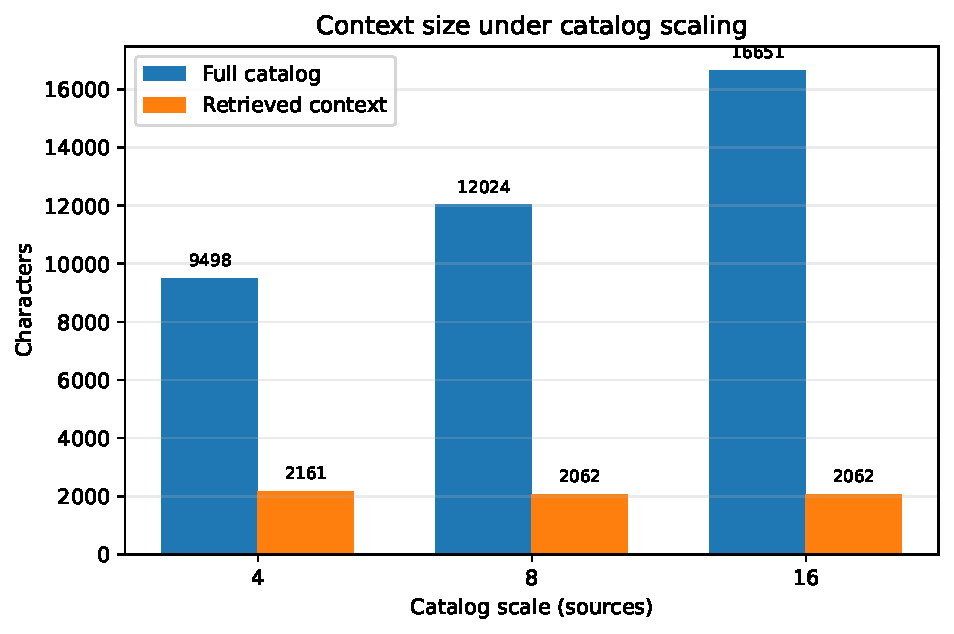
\includegraphics[
        width=0.78\textwidth
    ]{catalog_scale_context_size.pdf}
    \caption{
        Complete catalog size and mean relation-aware context size as the
        catalog grows from 4 to 16 sources.
    }
    \label{fig:catalog-context}
\end{figure}

The corresponding context reduction increases from 77.25\% at four sources to
82.85\% at eight sources and 87.62\% at sixteen sources.

However, this increased compression is accompanied by a retrieval-quality
trade-off. Macro recall decreases from 0.925 at four sources to 0.825 at eight
sources. Macro precision decreases from 0.662 to 0.620, and macro F1 decreases
from 0.754 to 0.683.

The number of perfect-recall held-out questions decreases from 17 out of 20 to
14 out of 20.

Figure~\ref{fig:catalog-recall} shows the recall trend.

\begin{figure}[htbp]
    \centering
    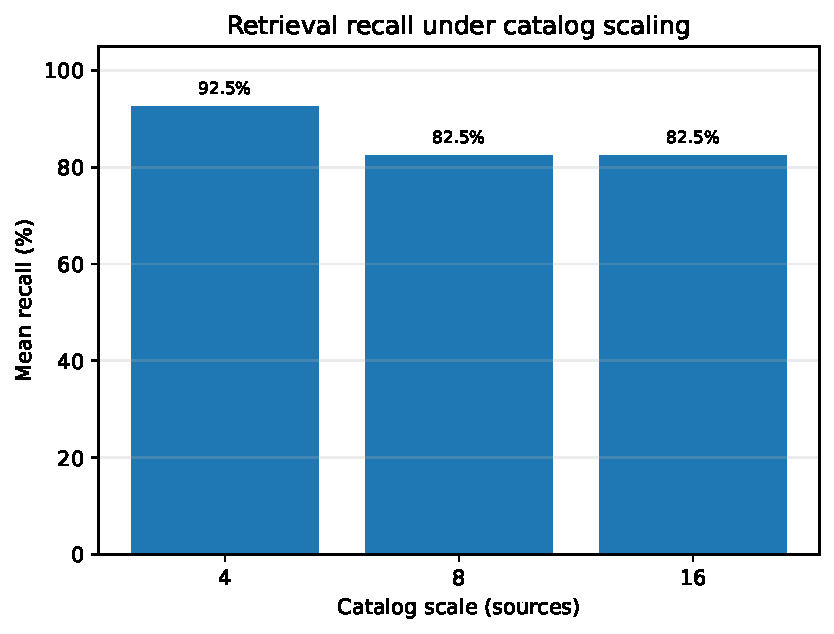
\includegraphics[
        width=0.68\textwidth
    ]{catalog_scale_recall.pdf}
    \caption{
        Mean metadata recall under increasing catalog scale.
    }
    \label{fig:catalog-recall}
\end{figure}

Importantly, no additional degradation is observed when the catalog grows from
8 to 16 sources. Recall, precision, F1, mean context size, and perfect-recall
count remain unchanged between these two scales.

The result therefore does not indicate a simple monotonic relationship in
which every additional source causes further degradation. Instead, particular
semantically similar hard negatives introduced at the eight-source scale are
responsible for the observed loss.


\subsection{Catalog-Scale Error Analysis}

Post-hoc analysis of the frozen catalog-scale results identifies the specific
metadata lost when the first hard-negative sources are introduced.

For both held-out variants of the Green Taxi drop-off borough query, retrieval
is perfect with four sources. At eight sources, the retriever loses:

\begin{itemize}

    \item \texttt{taxi\_zones};
    \item \texttt{taxi\_zones.Borough};
    \item \texttt{taxi\_zones.LocationID};
    \item the Green Taxi drop-off-to-zone relationship.

\end{itemize}

A similar effect appears for one Yellow Taxi pickup-borough query, where the
retriever loses the Taxi Zones dataset, the borough and location columns, and
the Yellow pickup-to-zone relationship.

The most difficult three-source paraphrase already had incomplete weather
retrieval at four sources. After the hard-negative catalog expansion, it also
loses the geographic Taxi Zones metadata.

These failures are consistent with semantic competition from the added
domain-related distractors, particularly sources containing borough,
geographic, weather, or alternative mobility concepts.

The fact that the same failures persist unchanged at sixteen sources suggests
that the observed degradation is caused mainly by the first set of strongly
competitive hard negatives rather than by catalog size alone.


\subsection{Metadata Index Construction Cost}

Catalog growth also increases the amount of metadata that must be embedded and
indexed.

With four sources, the index contains 103 metadata documents and requires
6,472 embedding prompt tokens. Index construction uses 28.54 seconds of
embedding wall time.

At eight sources, the index contains 131 documents, requires 8,437 embedding
tokens, and uses 30.68 seconds of embedding wall time.

At sixteen sources, the index grows to 188 documents and 11,585 embedding
tokens, with 42.43 seconds of embedding wall time.

These measurements represent index-construction cost rather than per-query
retrieval cost. Since metadata indexes can be reused across many analytical
requests, this cost is operationally different from the prompt and generation
cost incurred for each user query.


\subsection{Spark Data-Volume Scalability}

The final experiment evaluates the physical execution layer independently from
metadata-catalog growth.

Table~\ref{tab:data-volume-scaling} reports median Spark runtime across three
repetitions for each workload and data volume.

\begin{table}[htbp]
\centering
\caption{Spark data-volume scaling using median runtime over three repetitions.}
\label{tab:data-volume-scaling}
\begin{tabular}{lrrrrr}
\toprule
Scale & Rows & Parquet MiB & Scan (s) & Grouping (s) & Weather join (s) \\
\midrule
100k & 100,000 & 2.31 & 0.140 & 0.226 & 0.274 \\
500k & 500,000 & 11.44 & 0.140 & 0.293 & 0.406 \\
1m & 1,000,000 & 23.24 & 0.146 & 0.224 & 0.615 \\
Full & 2,963,713 & 72.58 & 0.199 & 0.492 & 1.350 \\
\bottomrule
\end{tabular}
\end{table}


The physical Yellow Taxi benchmark scales from 100,000 rows to the complete
2,963,713-row curated dataset. The corresponding two-file Parquet
representation grows from 2.31 MiB to 72.58 MiB.

Figure~\ref{fig:data-volume} presents the runtime curves.

\begin{figure}[htbp]
    \centering
    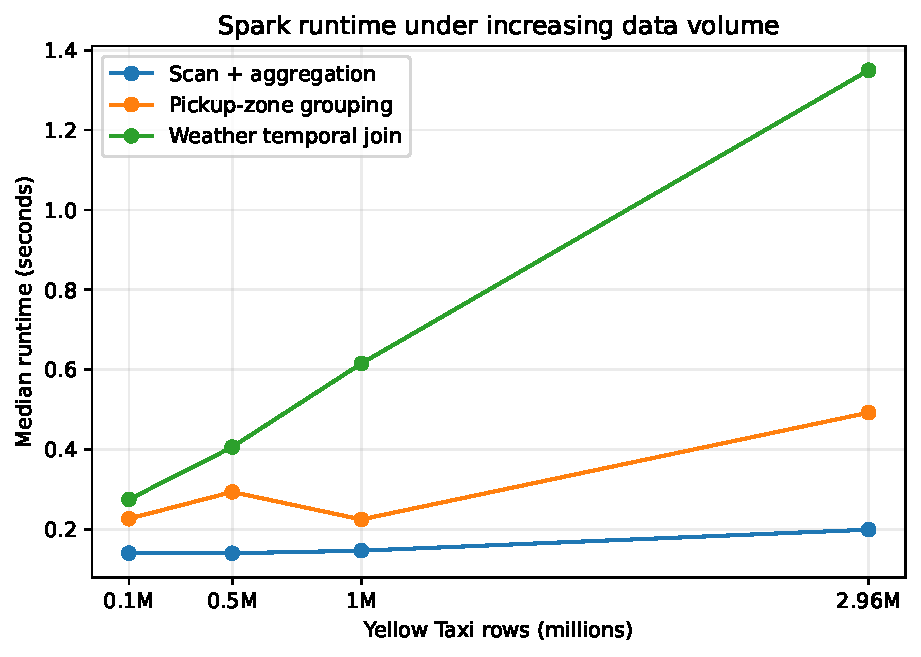
\includegraphics[
        width=0.80\textwidth
    ]{spark_data_volume_scaling.pdf}
    \caption{
        Median Spark runtime under increasing Yellow Taxi data volume.
    }
    \label{fig:data-volume}
\end{figure}

For the simple scan-and-aggregation workload, median runtime is 0.140 seconds
at 100,000 rows and 0.199 seconds for the complete dataset. The corresponding
runtime factor is 1.42 despite an approximately 29.6-fold increase in row
count.

The pickup-zone grouping workload increases from 0.226 seconds to
0.492 seconds, corresponding to a 2.18-fold runtime increase.

The temporal taxi--weather join shows the clearest volume-dependent growth.
Median runtime increases from 0.274 seconds at 100,000 rows to 0.406 seconds
at 500,000 rows, 0.615 seconds at one million rows, and 1.350 seconds for the
complete dataset. The full-data runtime is 4.92 times the 100,000-row
baseline.

The first repetition of several small workloads is substantially slower than
later repetitions, confirming the presence of JVM, filesystem, and execution
warm-up effects. For this reason, the pre-defined benchmark reports the median
of three runs rather than interpreting a single execution.


\subsection{Interpretation of the Scaling Results}

The data-volume experiment should not be interpreted as evidence that Spark
has a universally sub-linear runtime curve. The maximum test dataset is only
72.58 MiB in its materialized Parquet representation and is executed using two
local worker threads.

At the smaller scales, fixed costs such as query planning, task scheduling,
JVM warm-up, and filesystem caching can dominate the actual scan cost. This is
particularly visible in the simple aggregation workload.

The temporal weather join provides a clearer scaling signal because it
performs additional timestamp transformation and cross-source matching.

The main conclusion from this experiment is therefore limited and
implementation-specific: the prototype successfully executes the selected
analytical workloads from 100,000 rows to the complete 2.96-million-row
Yellow Taxi dataset, while the measured runtime remains manageable in the
two-core experimental environment.


\subsection{Summary of Main Findings}

The experimental results provide four main findings.

First, relation-aware SQL-safe metadata retrieval improves held-out result
accuracy from 70\% to 80\% relative to complete-catalog prompting, and
validation-driven one-shot repair further increases accuracy to 85\%.

Second, the relation-aware context reduces mean prompt size by 69.66\% and
reduces controlled prompt-evaluation time by 70.29\% in the CPU-only
experimental environment.

Third, relation-aware retrieval keeps prompt context approximately bounded as
the metadata catalog grows, but semantically related hard negatives introduce
a measurable recall trade-off. Macro recall decreases from 0.925 to 0.825
when the first distractor sources are introduced, then remains stable as the
catalog grows further.

Fourth, the Spark execution layer successfully handles the evaluated
data-volume range up to 2,963,713 curated Yellow Taxi records, with the
temporal weather join exhibiting the clearest increase in runtime as volume
grows.

These findings are examined further in the discussion of system benefits,
limitations, and failure modes in Section~\ref{sec:discussion}.

\section{Discussion}
\label{sec:discussion}

\subsection{Interpretation of the Main Result}

The experiments support the central hypothesis of the project: metadata
selection is not merely a prompt-compression mechanism. In the evaluated
setting, a smaller relation-aware and SQL-safe context produces better
held-out results than complete-catalog prompting while also reducing model
input cost.

The central interpretation is therefore qualitative as well as quantitative.
The language model benefits when semantic descriptions are preserved but
internal metadata identifiers and unrelated schema elements are prevented
from competing with the physical Spark objects needed for execution.


\subsection{Why the Complete Catalog Can Underperform}

At first sight, the complete catalog should appear advantageous because it
contains all information needed to answer every benchmark question. However,
the experiments show that information availability and information usefulness
are not equivalent.

The full catalog includes physical schema elements together with semantic
concepts, aliases, relationship identifiers, and rule identifiers. These
metadata objects are useful internally, but they are not all valid SQL table
or column names.

An LLM exposed to the complete catalog must therefore distinguish between
physical identifiers and descriptive metadata while simultaneously solving
the analytical task. The held-out failures show that the model can incorrectly
promote an internal semantic identifier into generated SQL.

The SQL-safe relation-aware renderer removes much of this ambiguity. It keeps
semantic meaning available through descriptions while exposing only physical
tables, columns, join conditions, and executable expressions as SQL objects.

The advantage of Configuration B therefore comes from both
\emph{selection} and \emph{representation}: less metadata is shown, and the
metadata that remains is presented in a form that more directly matches the
execution language.


\subsection{Retrieval Completeness and SQL Accuracy}

One of the clearest findings is the association between metadata recall and
downstream query correctness.

For held-out questions with perfect metadata recall, the relation-aware
configuration achieves 88.2\% result accuracy, while the validation-and-repair
configuration reaches 94.1\%.

For questions with imperfect metadata recall, accuracy drops to 33.3\% for
both configurations.

This difference is expected from the system architecture. The LLM can only
generate a correctly grounded cross-source query if its prompt contains the
physical datasets, columns, relationships, and semantic rules needed to
express that query.

When required metadata is missing, the model may invent a plausible schema
element or simplify the query so that an intended source is omitted. Such
errors cannot always be detected from syntax alone.

This suggests that metadata recall is a critical upstream metric for
metadata-aware Text-to-SQL systems. High retrieval precision is useful for
keeping prompts compact, but insufficient recall can directly remove
information required for executable query construction.


\subsection{Limits of Semantic Similarity}

The catalog-scale experiment highlights a limitation of dense semantic
retrieval.

At four sources, the relation-aware retriever achieves macro recall of 0.925.
After four domain-related hard-negative sources are introduced, macro recall
drops to 0.825.

The error analysis shows that the new failures are not random. They are
concentrated around geographic metadata, especially Taxi Zones relationships
and borough-related fields.

This result illustrates a general challenge in metadata retrieval:
semantically similar sources can compete for a small Top-\(k\) retrieval
budget even when only one source has the correct structural relationship
required for execution.

The deterministic relation-expansion stage mitigates this problem only after
the relevant dataset or concept has been selected. If dense and lexical
retrieval fail to provide enough evidence for the correct dataset in the
first place, later relationship expansion cannot reliably recover it.

The experiment therefore shows that semantic similarity and structural
correctness are complementary rather than interchangeable.


\subsection{Catalog Growth and Bounded Context}

A positive scalability result is that relation-aware context size remains
approximately bounded while the full catalog grows substantially.

The complete catalog grows from 9,498 to 16,651 characters between four and
sixteen sources. The retrieved context remains near 2,100 characters.

This behaviour is desirable because the per-query prompt does not need to
scale linearly with total metadata volume.

However, the corresponding increase in context reduction must not be
interpreted in isolation. At eight and sixteen sources, part of the greater
compression is associated with missing required metadata.

The correct interpretation is therefore a trade-off: relation-aware retrieval
successfully decouples prompt size from catalog size, but aggressive selection
can reduce recall when hard negatives compete with the correct metadata.

A production system would need to manage this trade-off explicitly, for
example by using adaptive retrieval depth, stronger structural reranking, or
confidence-aware expansion.


\subsection{Interpreting the 8-to-16 Source Plateau}

An interesting aspect of the catalog-scale experiment is that performance does
not continue to degrade when the catalog increases from eight to sixteen
sources.

Macro recall, precision, F1, perfect-recall count, and mean context size are
identical at these two scales.

This suggests that catalog size alone is not the main cause of the observed
failure. Instead, the first group of hard negatives contains metadata that is
particularly competitive with the intended sources.

The additional eight sources increase the total catalog substantially but do
not introduce new retrieval errors for the frozen benchmark.

This distinction matters because it prevents an overly broad conclusion such
as ``retrieval quality decreases as the number of sources increases.'' The
results support a more precise statement: retrieval quality can degrade when
new sources are semantically similar enough to displace structurally required
metadata.


\subsection{Effectiveness and Limits of Validation}

SQL validation provides a useful safety boundary between the language model
and Spark execution.

The validator can detect unknown physical columns, invalid relations,
syntactic problems, incompatible expressions, and unexpected output
structures before a query is executed.

This protects the execution layer from a class of common LLM generation
errors. It also provides actionable feedback that can be passed to the repair
stage.

However, validation cannot establish full semantic correctness.

A valid query may still use the wrong filter, choose the wrong dataset,
produce a different categorical convention, or express a related but
incorrect analytical computation. These queries may pass parsing and Spark
analysis while returning an incorrect benchmark result.

For this reason, the project treats result accuracy as the primary correctness
metric rather than validation rate.


\subsection{Effectiveness and Limits of One-Shot Repair}

The repair stage provides a measurable but limited improvement.

Three held-out queries triggered repair, and one repair produced a validated
and correct result. This raises overall result accuracy from 80\% to 85\%.

The successful case demonstrates the intended role of repair: the necessary
metadata was already available, the generated query contained a physical
schema error, and validator feedback gave the model enough information to
correct the query.

The failed repair cases reveal the opposite condition. When retrieval omitted
essential weather or relationship metadata, the repair model was given no new
source of structural knowledge. A validation error can identify that a column
does not exist, but it cannot reliably reconstruct an omitted multi-source
relationship.

One-shot repair is therefore best understood as a local correction mechanism,
not as a substitute for metadata retrieval.


\subsection{Prompt Reduction and Latency}

The relation-aware context reduces mean held-out prompt size by 69.66\%.

The controlled latency benchmark shows a similar reduction in prompt
evaluation cost: mean prompt-evaluation time decreases by 70.29\% under the
prefix-isolated protocol.

The similarity between these reductions is consistent with the expectation
that shorter prompts require less input processing by the language model.

The original sequential held-out timings, however, show why LLM latency must
be measured carefully. Repeated complete-catalog prompts share a large common
prefix and can benefit substantially from runtime cache behaviour.

Without the controlled benchmark, these cache effects could lead to the
incorrect conclusion that the larger full-catalog prompt is intrinsically
faster.

The separate prefix-isolated and natural-cache measurements therefore improve
the reliability of the efficiency analysis.


\subsection{Interpretation of the Spark Scaling Experiment}

The Spark data-volume experiment confirms that the complete analytical
pipeline can execute over progressively larger physical datasets, up to
2,963,713 curated Yellow Taxi records.

The temporal weather join shows the clearest runtime growth, increasing from
0.274 seconds at 100,000 rows to 1.350 seconds at full scale.

The simpler workloads show weaker monotonic behaviour because the experimental
datasets remain small enough for fixed execution costs and local caching
effects to be significant.

The results therefore demonstrate feasibility and relative behaviour within
the selected environment, but they should not be used to claim general Spark
scalability properties.

A distributed cluster experiment with substantially larger physical data
would be required to evaluate network shuffle, executor scaling, partitioning
strategy, and cluster-level resource utilisation.


\subsection{Big Data Perspective}

The project addresses the Big Data dimensions of Volume and Variety in
different parts of the system.

Volume is handled by Spark and evaluated by increasing the number of taxi
records processed by the physical execution layer.

Variety is handled primarily by the metadata architecture. Different physical
schemas, naming conventions, source roles, geographic joins, and temporal
granularities are represented explicitly in the catalog.

The experiments show that these two dimensions create different engineering
problems. Increasing row volume affects execution cost, whereas increasing
metadata variety affects grounding ambiguity and prompt construction.

Separating catalog scale from data scale is therefore useful when analysing
data-centric generative-AI systems: a system can scale well in physical query
execution while still failing because metadata grounding becomes ambiguous.


\subsection{Threats to Validity}

Several factors limit the generality of the experimental results.

First, the held-out benchmark contains 20 questions derived from ten analytical
intents. Although the natural-language paraphrases were frozen before final
evaluation, the benchmark remains small compared with large public
Text-to-SQL datasets.

Second, all core data comes from a single application domain: New York City
mobility and weather. The architecture may behave differently with metadata
from unrelated enterprise domains.

Third, the local language model is relatively small and executed without a
GPU. Larger models may have different sensitivity to metadata noise and may
require different retrieval depths.

Fourth, the catalog-scale distractors are synthetic metadata-only sources.
They are deliberately designed as hard negatives, but they do not reproduce
all characteristics of a large production catalog.

Fifth, the physical Spark evaluation is local rather than distributed and
reaches approximately three million rows. It therefore demonstrates prototype
behaviour rather than cluster-scale performance.

Finally, result correctness depends on the benchmark's expected-result and
comparison procedure. Some analytically equivalent outputs may differ in
labels or formatting, as observed in one cross-taxi comparison.


\subsection{Possible Improvements}

Several extensions could address the observed limitations without changing the
core design.

Retrieval could use an adaptive Top-\(k\) rather than a fixed value of five,
increasing metadata coverage when retrieval confidence is low.

A structural reranking stage could explicitly favour datasets connected by
catalog relationships required by the candidate analytical intent.

Retrieval confidence could also be exposed to the downstream pipeline. When
required metadata is uncertain, the system could request additional metadata
before generation rather than relying on repair after SQL failure.

The metadata catalog could be expanded with richer type constraints,
cardinality information, data-quality statistics, and source-level
provenance.

For larger deployments, the local SQLite and embedded Qdrant components could
be replaced by distributed metadata and vector services while preserving the
same logical interfaces.

Finally, repair could be extended beyond one attempt, although any iterative
strategy would require careful control to avoid uncontrolled agent loops and
to preserve reproducibility.


\subsection{Overall Assessment}

The prototype demonstrates that a relatively small local language model can
perform useful cross-source Spark SQL generation when it is supported by
explicit metadata grounding.

The key result is not that retrieval always succeeds. The catalog-scale
experiment shows clear cases in which hard negatives reduce recall.

Rather, the project demonstrates that the way metadata is selected and
rendered has a measurable effect on correctness, prompt size, and inference
cost.

The architecture therefore supports a data-centric interpretation of
Text-to-SQL: improving the representation and delivery of metadata can be as
important as changing the language model itself.

\section{Conclusions and Future Work}
\label{sec:conclusions}

This project investigated whether metadata-aware retrieval can improve
Text-to-Spark-SQL generation over a heterogeneous data lake.

The implemented prototype combines a structured metadata catalog, local
semantic embeddings, relation-aware metadata retrieval, SQL-safe context
rendering, a local language model, SQL validation, optional one-shot repair,
and Apache Spark SQL execution.

The central design choice is to avoid providing the complete metadata catalog
to the language model for every request. Instead, the system retrieves and
expands only the metadata considered relevant to the current analytical
question, while explicitly preserving physical datasets, columns,
relationships, and semantic rules required for execution.

The experimental results support this approach.

On the frozen held-out benchmark, complete-catalog prompting achieved 70\%
result accuracy. Relation-aware metadata retrieval increased result accuracy
to 80\%, and the addition of validation-driven one-shot repair increased it
further to 85\%.

At the same time, relation-aware prompting reduced mean prompt size from
2558.45 to 776.35 tokens, corresponding to a 69.66\% reduction. In the
controlled CPU-only latency experiment, mean prompt-evaluation time decreased
from 182.58 seconds to 54.24 seconds, a reduction of 70.29\%.

The catalog-scale experiment showed that the retrieved context remains
approximately bounded while the complete metadata catalog grows. The full
catalog increased from 9,498 characters with four sources to 16,651
characters with sixteen sources, while the mean retrieved context remained
close to 2,100 characters.

This scalability benefit is accompanied by an important limitation. Macro
metadata recall decreased from 0.925 to 0.825 after semantically related
hard-negative sources were introduced. Error analysis showed that the
degradation was caused primarily by competition around geographic and weather
metadata rather than by catalog size alone.

The held-out results also demonstrated the importance of retrieval
completeness. Queries with perfect metadata recall achieved substantially
higher downstream result accuracy than queries with missing required
metadata. Validation and repair can correct some invalid SQL generations, but
they cannot reliably compensate for relationships or schema information that
were never retrieved.

The Spark data-volume experiment evaluated the physical execution layer from
100,000 rows up to the complete 2,963,713-row curated Yellow Taxi dataset.
The temporal taxi--weather workload showed the clearest runtime growth, while
the simpler workloads were strongly influenced by fixed execution and warm-up
costs in the two-core local environment.

Overall, the results suggest that metadata management is a central component
of data-centric generative-AI systems for structured analytics. Improving the
way metadata is selected and represented can improve both correctness and
efficiency without changing the underlying language model.

Future work could extend the prototype in several directions.

First, retrieval could use an adaptive Top-\(k\) strategy or confidence-aware
expansion rather than a fixed dense retrieval depth. This could improve recall
when semantically similar catalog sources compete for the same retrieval
budget.

Second, structural reranking could make stronger use of catalog relationships,
schema compatibility, cardinality information, and expected analytical
operations before the final context is rendered.

Third, the metadata catalog could incorporate richer provenance, data-quality
statistics, source freshness, and additional semantic constraints.

Fourth, the evaluation could be expanded to larger and more diverse
cross-domain benchmarks, including catalogs that contain substantially more
physical sources and unrelated business domains.

Fifth, the Spark execution experiment could be repeated on a distributed
cluster and with much larger physical datasets in order to study partitioning,
shuffle behaviour, executor scaling, and resource utilisation.

Finally, larger or alternative local language models could be evaluated using
the same frozen metadata and benchmark infrastructure. This would make it
possible to separate improvements caused by stronger language models from
those caused by better metadata grounding.

The main contribution of the project is therefore not a claim that
relation-aware retrieval eliminates Text-to-SQL errors. Instead, the project
provides a reproducible demonstration that metadata selection, structural
expansion, SQL-safe representation, validation, and controlled evaluation can
substantially influence the behaviour of language-model-based analytics over
heterogeneous Big Data sources.



% ---------------------------------------------------------
% Bibliography
% ---------------------------------------------------------

\clearpage

\bibliographystyle{plain}
\bibliography{references}


% ---------------------------------------------------------
% Appendix
% ---------------------------------------------------------

\clearpage
\appendix

\section{Reproducibility and Experimental Freeze Protocol}


\end{document}
